\chapter{Monitoring Application Energy Usage During Operation}

% Explain the problem we're trying to solve and the model for allocating it.


\section{Introduction}

The energy usage of information and communications technology (ICT) systems is starting to receive much more attention that it has historically.  This is due to the sharply increasing demand for electricity to run the digital economy, with US datacenters alone consuming an estimated 91 billion kWh in 2013 and are expected to consume 140 billion kWh by 2020 \cite{delforge2014-datacentreenergy}.

Researchers have been working for some years to understand the energy demand of ICT systems and significant progress has been made in a number of areas.  At the macro level, understanding how data centres use power and reducing the amount of power required in the data centre environment [REF].  At the micro-level, there have been some promising steps in understanding how individual programs consume power, to the point where it is possible to quite accurately predict and compare the power consumption of different options for program implementation [REF].

The problem for the software engineering practitioner is that their interest sits between these two extremes as they need to understand the energy consumption at the overall application level rather than at the individual component level or at the data centre level where many applications are consolidated.

The modern trend towards microservice-based systems [REF] makes things more complicated for the practitioner.  While it was possible to see ways of using program energy estimation approaches with monolithic applications, this quickly becomes overwhelming with a microservice-based system, due to the number of possible pieces of the system that could be involved in processing a workload or request.

In this chapter, we present the design for a piece of technology that we have designed to address this problem by fairly allocating the energy usage of a host machine to the application elements running on it.  Using modern microservice and operating system technology including containers, tracing and resource monitoring, combined with energy statistics for a machine, we can provide the host operator and the software architect with reliable estimates of the energy allocation of a machine's total consumption required to process requests for an application running on it.  This allows cost estimation and the evaluation of architectural alternatives to minimise energy consumption.

\section{Motivation}

There are several reasons to seek a method of estimating energy usage by software applications, but two immediate motivating examples in our case are cost estimation and architectural evaluation.

Today, the energy consumption of an application is not taken into account when considering its cost to operate and so there is little motivation for the software architect to understand and minimize their application's energy footprint.  This prevents large possible reductions in energy usage and its associated resources of environmental impact and cost.

Even where the architect is interested in the energy usage of their application, no mainstream and practical approach for estimating the energy usage of software at the application level is available.  This means that for applications where a significant number of system elements are used to process a request, as in a microservices-based system, it theoretically possible to use program-level approaches to estimate the energy usage, but is complex enough that we do not believe that it is done in practice.  This means that architects cannot evaluate the energy usage qualities of different architectural options.

The specific advanced achieved by this piece of work is the design an approach to measuring resource usage for request processing in a distributed application in such a way that an energy model can be used to estimate the energy usage of specific requests made to the application.

The goal of this is to provide a practical approach for software architects to estimate the energy costs of their applications and to evaluate different architectural options in terms of their likely energy usage.

\section{Microservice-Based Systems}

The microservice architectural style [REF] is rapidly becoming a mainstream approach for building industrial software systems and it is systems build using this style that we are specifically interested in for this work.
A microservice-based system is made up of many small, encapsulated, network-connected services, rather than the more traditional approach of having a small number of large servers that aggregated many services (a so-called "monolith" [REF]).

For our purposes, the important characteristics of a microservice-based system are:

\begin{itemize}
\item The business logic in the system is implemented as a group of small, focused services, each performing one task, typically implementing a "bounded context" in Domain Driven Design terms [REF].
\item The services are as independent as possible and have well defined service interfaces and only interact through these interfaces.  Resources such as databases are owned by a specific service and are not accessed by other services (hence a microservice-based system will have many independent data stores rather than a single consolidated database used by many services).
\item Handling an incoming request for a system is likely to involve a set of cooperating services, with one handling the initial request and then calling other services in order to fulfil the request and provide a response.  Microservice-based systems often separate request-handling and domain services but we do not assume that this is necessarily the case.
\end{itemize}

Well designed microservice-based systems typically share other important characteristics [REF], such as independent build, test and deploy for each service, and interfaces defined using machine readable formats such as Swagger [REF] and RAML [REF] but these other characteristics are not significant in the context of this work, and so we do not assume that they are present.

\section{Estimating Energy Usage}

As we investigated the problem of how to provide software architects, and other interested parties like data centre operators, with estimates of application level energy usage we identified a number of possible approaches.  

\begin{itemize}
\item Other researchers have tried to create entirely \emph{model based approaches} (such as [REF]) which can allow relative energy usage between different architectural structures to be estimated, but sidestep the problem of calculating actual energy values and require significant amounts of effort to create the models for non-trivial applications.

\item Other research projects have attempted to estimate architectural characteristics through \emph{event based simulation} but creating event based simulation models is an unfamiliar process to many practitioners and again is significant amounts of effort for non-trivial systems.  It is also the case that existing research in this area has not yet investigated how to estimate energy consumption, but rather has focused on other architectural qualities such as performance.

\item At the \emph{micro-measurement level}, sophisticated approaches have been designed to estimate energy consumption for individual algorithms or programs [REF-JOLINAR] with a high degree of success.  However these approaches rely on a highly controlled execution environment for the code being measured and access to low-level hardware state metrics, such as processor frequency statistics, in order to deal with the complex power characteristics of modern computing hardware.  While these models and tools are undoubtedly useful in the right situation, they are not practical tools for measuring the energy usage of a large-scale modern distributed application.

\item We explored whether we could combine the \emph{micro-measurement} approaches with \emph{application-level resource usage estimation} and produce meaningful energy estimates for the application-level workload.  However we found that approaches like Jolinar are not effective unless the low-level hardware state metrics can be provided and this wasn't practical in large distributed execution environments such as those used by microservice-based systems.

\end{itemize}

Having considered these options and realised that each of them had severe practical limitations, we shifted our focus slightly and reconsidered the goal of the work.  The problem we aimed to solve was to provide software architects and other interested parties with information on how to improve the energy efficiency of their applications.  The solution we identified to this problem was to shift our  goal from precisely estimating the \emph{actual} energy usage of a distributed application to estimating the \emph{fair allocation} of energy consumption to the application.  This is a useful goal because it allows service providers (such as cloud or hosting operators or data centre operators) to fairly allocate the cost of energy consumed by their infrastructure and it allows software architects to understand the energy consumption implications of their design decisions in relative terms, even if not in absolute energy consumption terms.

Our approach assumes that the energy consumption of the execution platform that the application is executing on is available to the energy calculation process and uses this, along with the total resource usage consumption of the execution platform and the resource usage of the application components to allocate the platform energy consumption to the different application elements running on it.  By tracing the execution of inbound requests across application elements, this allows us to allocate energy usage to specific requests and so compare the energy efficiency of different parts of a system and different design options for a system.

Estimating energy usage at the application level is a complex process and so it is important to be clear how the calculation will be performed before trying to design an implementation of it.

There are five quite distinct parts to the problem:

\begin{itemize}

\item \emph{Identification of service elements involved in processing a request}.  Processing a request in a modern distributed system will often involve a chain of service calls between the services that comprise the system logic.  We assume that the implementation of the services is under the control of those wishing to estimate energy consumption.

\item \emph{Identification of the processing periods attributable to a request}.  Once we know the system elements involved in processing a particular request, we need to identify when the element was performing work on behalf of the request.

\item \emph{Resource usage of the request}.  Given the system elements involved in processing a request and the periods when they were active, on behalf of the request, we need to estimate the runtime resources consumed by the system elements during these periods.  The resource consumption we need to estimate is the amount of CPU consumed, the amount of active memory in use, the number of network i/o bytes sent and received, and the number of disk i/o bytes read and written.

\item \emph{Estimation of resource and energy usage of the underlying host machine}.  Our aim is to fairly allocate the energy used by a machine during a time window across the requests that were active during that period.  Hence we need to estimate the overall resource usage of the machine and the energy that it consumed as a result.

\item \emph{Energy estimate of the request}.  Once we have the resource consumption metrics for a particular request, we then need to translate these into an estimate of the energy consumption that they imply.  We do this by establishing the percentage of overall machine resource utilisation that can be attributed to the request and then allocating the same percentage of energy usage of the underlying host to the request.

\end{itemize}

Each of these aspects of the problem has their own complexities, but they can largely be solved independently, and once resolved, it will be possible to achieve a reliable and fair energy allocation for each inbound request for a microservice-based system.  In the following sections of this chapter we discuss how each of these aspects of the problem can be implemented.

\section{Logical Design of an Energy Estimation System}

The functional design of a system to estimate energy usage for application requests (which we have dubbed "Apollo" - the Greek God of Prophesy, amongst other things [REF]) is shown in the informal block diagram in \ref{figure:logicaldesign}.

\begin{figure}
\centering
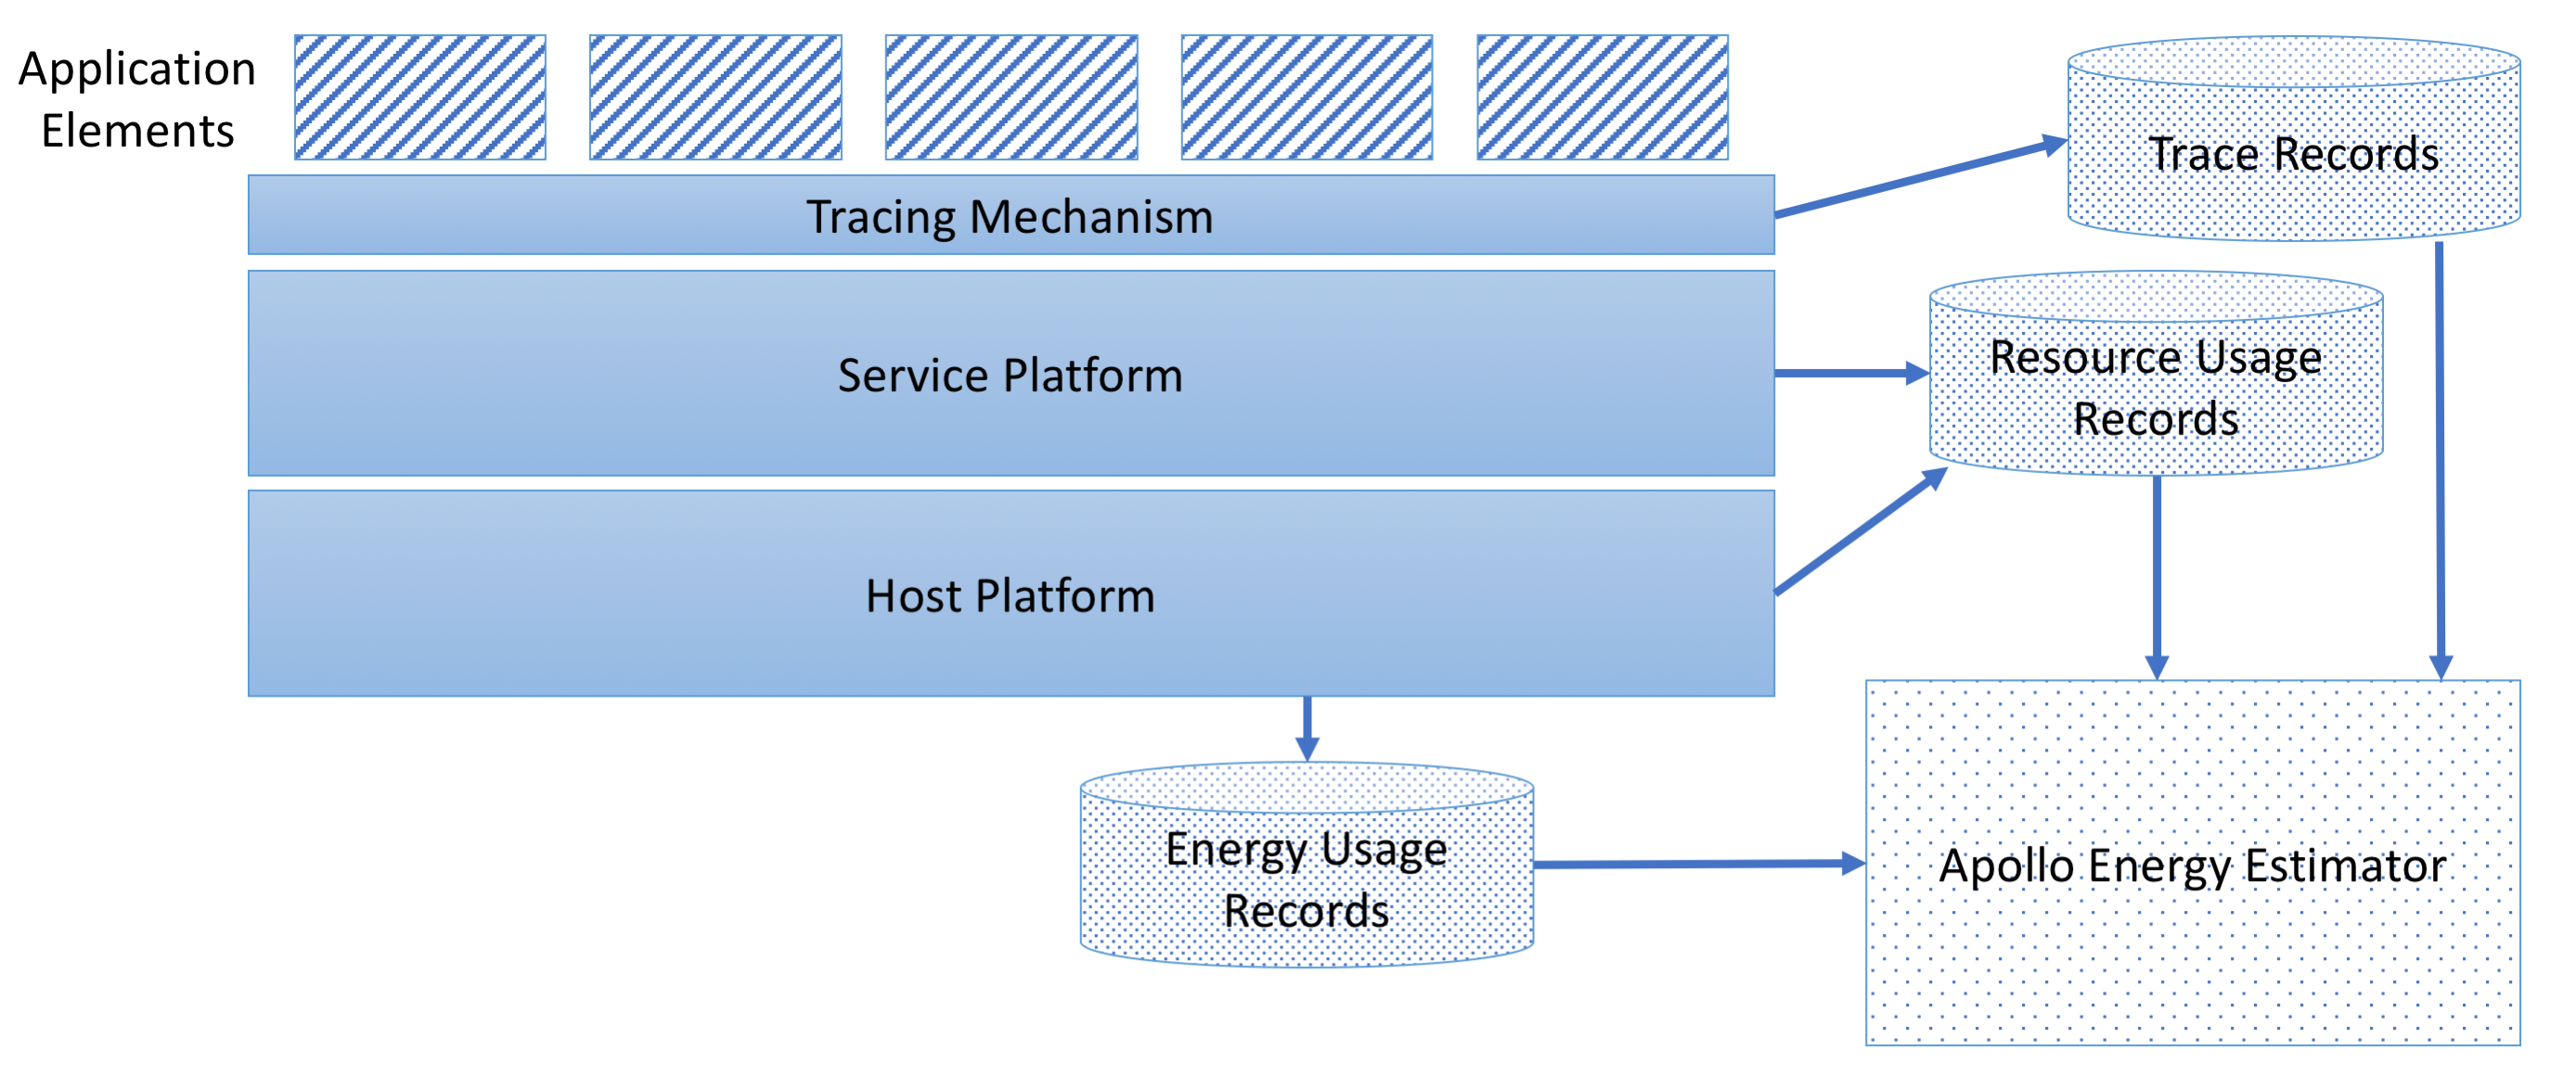
\includegraphics[width=\textwidth]{Figures/estimating-energy-logical}
\caption{Logical Design of the Energy Estimation System 'Apollo'}
\label{figure:logicaldesign}
\end{figure}

The elements in the diagram with solid fill are the underlying runtime platform and services, the diagonally hatched elements are the application under study, the densely-dotted elements are data, while the sparsely dotted elements are the Apollo energy estimation elements.

The elements of the system are briefly described below:

\begin{itemize}
\item \emph{Application Elements} are the architectural elements of the application which is being studied for energy consumption.  These are the main functional processing elements of the system, running in their own address space, providing a network interface to their services, invoked as part of request processing, with the implementation being under the control of the system owner who wants to estimate energy usage.  An example would be a request handling microservice to create an order.
\item \emph{Service Platform} is the system software which hosts the application components and can provide detailed measurements of their resource usage.  An example might be a PaaS platform like Cloud Foundry, a virtual machine or a container platform like Docker.
\item \emph{Host Platform} is the hardware and operating system platform that provides the general computing platform that hosts the service platform and provides runtime statistics on the platform's execution and energy consumption.
\item \emph{Tracing Mechanism} is key to our approach is the ability to trace which architectural elements were involved in handling a particular request for the system.  This tracing mechanism provides that ability, reporting the sequence of invocations of architectural elements and the time and duration of each.  Examples would be Zipkin and Jaeger.
\item \emph{Resource Usage Records} is a database of resource usage statistics for all of the functional elements of the system, fed from the Service Platform and the Host Platform.  An example could be Prometheus or InfluxDB, populated using a statistics collection server like Telegraf or cAdvisor.
\item \emph{Trace Records} is a database containing the request invocation traces from the Tracing Mechanism, which is likely to be a simple relational or document-oriented database, which the Tracing Mechanism writes its trace records to.
\item \emph{Apollo Energy Estimator} provides the key element of the energy estimation process, a calculator that works through the Trace Records and for each one, calculates which elements were active over which time periods, and uses the resource usage records to estimate the resource consumption of each request across the elements that were involved in processing the request.  These values are then compared with the overall host platform resource usage and the ratio of the values used to allocate the energy consumption of the host platform during the time period that the requests were active.

\end{itemize}

There are three key data structures in the design, which are critical to achieving the energy calculation, namely Trace Records, Resource Usage Records and Energy Usage Records.

\begin{itemize}

\item \emph{Trace Records} are created by the tracing mechanism and are used to record the invocation of system elements in processing a request.  There are two types of trace records, Traces and Spans.  Common features of the two are the identity of the runtime element writing the record, the start time of the record and the end time of the record.  A "trace" is written by the first element to handle an inbound request and its start time is when the request is received and its end time is when the response was dispatched.  A "span" records the activity of a single element in the handling of a request and it has a "parent" attribute which indicates the trace it is part of.  Should an element \emph{e1} cause another element \emph{e2} to be invoked, then the span recording the start and end times of the \emph{e2} activity has the \emph{e1} span as its parent.  Hence traces and spans are organized into a tree that mirrors the invocation structure of the request handling.  An example trace is shown in \ref{figure:span}.

\begin{figure}
\centering
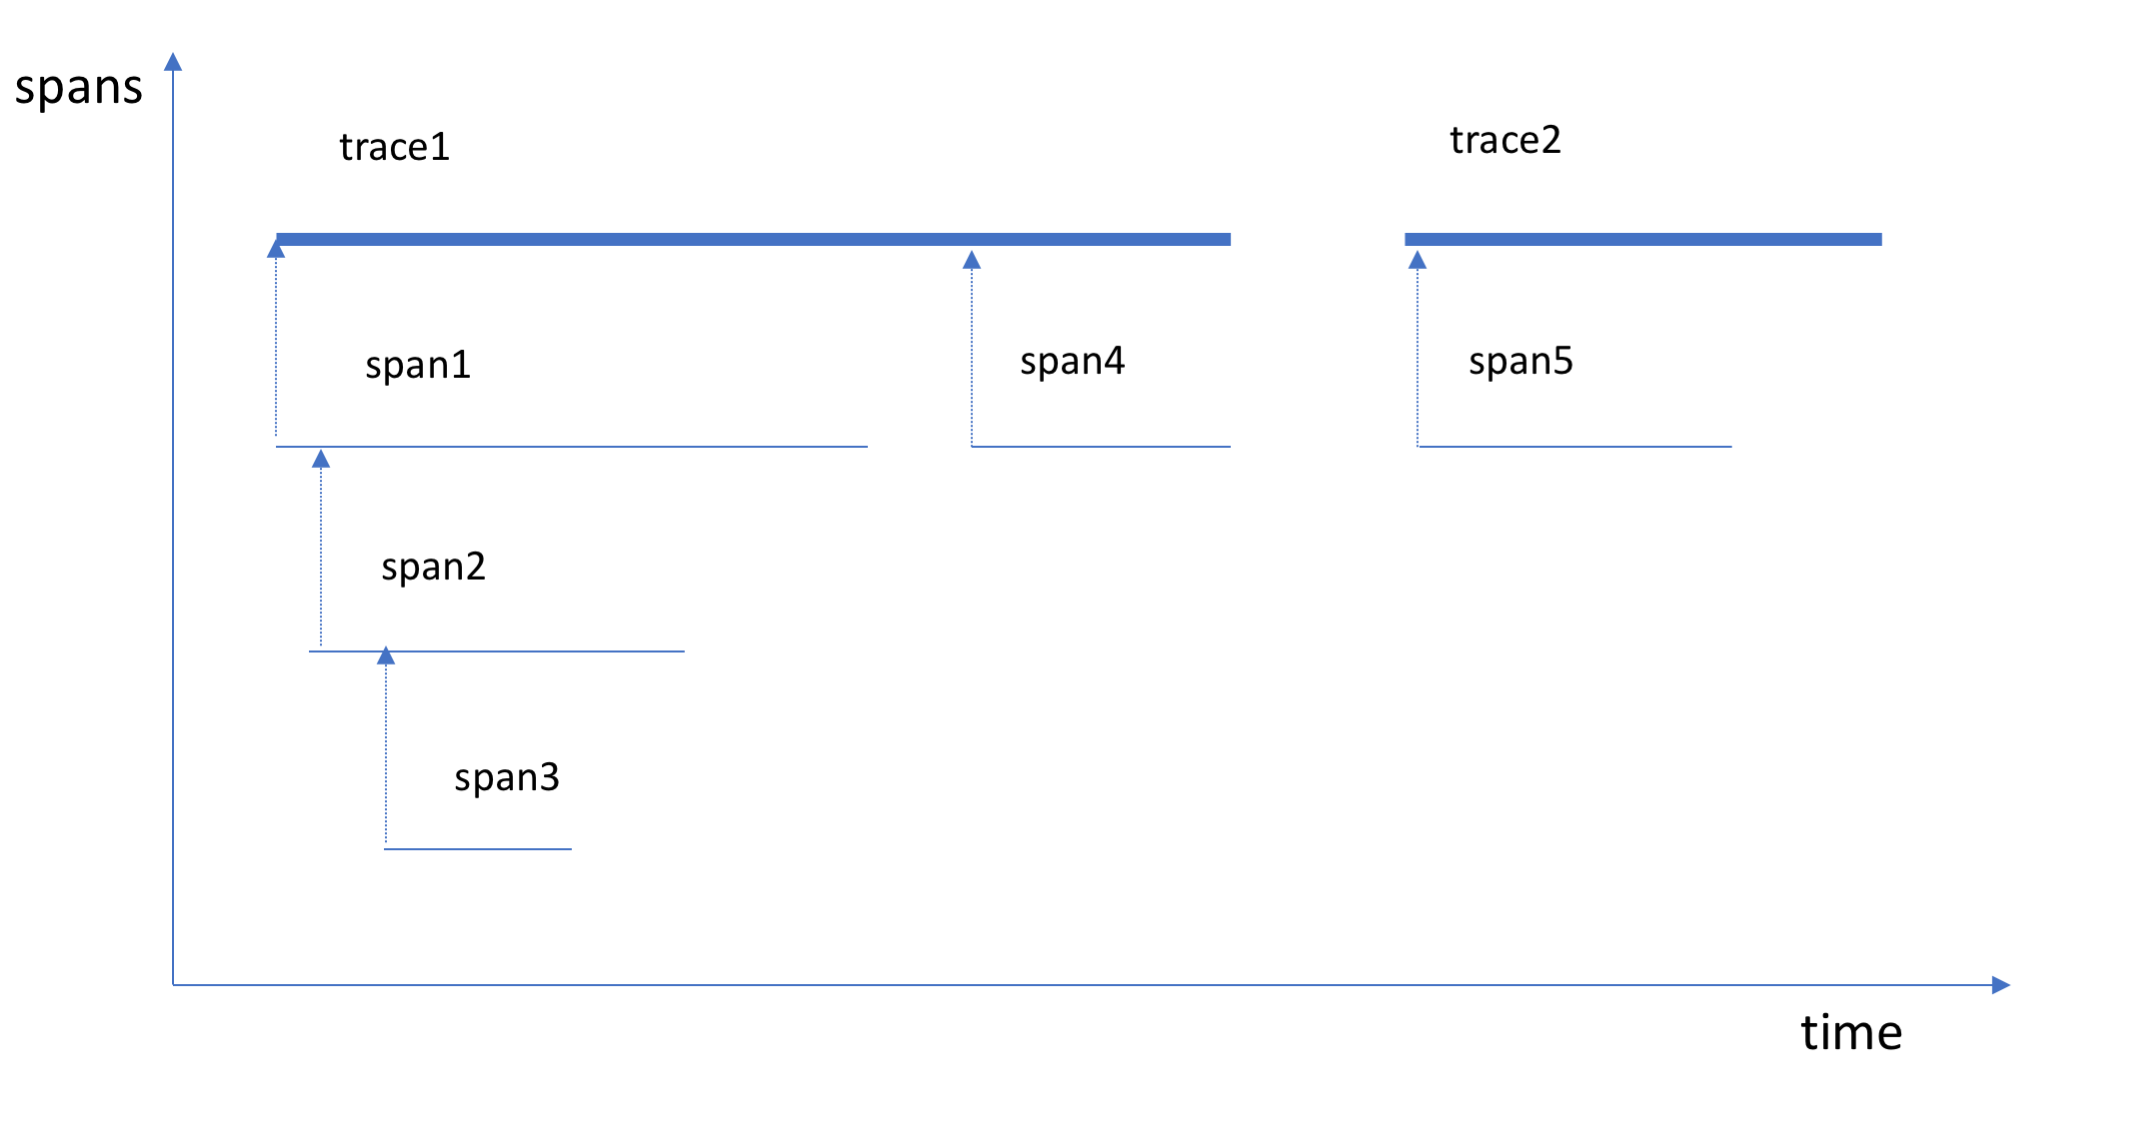
\includegraphics[width=0.75\textwidth]{Figures/estimating-energy-trace}
\caption{Example Execution Trace}
\label{figure:span}
\end{figure}

The figure shows two traces, representing requests, one after the other.  The traces are distinguished by not having parent spans, both traces have child spans, as indicated by the dotted arrows.  The y axis indicates invocation from top to bottom, the x axis indicates the passage of time.  The first request has two child spans, indicating that it invokes two other services.  Child span "span1" in turn invokes a third service, which invokes a fourth.  The second request invokes a single service.

\item \emph{Resource Usage Records} are generated by the runtime platform and stored in a timeseries style database to allow the metrics for a particular runtime element during a specified period to be retrieved (e.g. metrics for container c1 for the 3 second period from 20171105T084512.500 to 20171105T084515.500).  The metrics will be generated by the platform at regular but arbitrary intervals and so this data store will need to interpolate between the available measurement points to get the resource usage for the requested time periods.  The metrics that the runtime platform will be assumed to create are CPU usage (in "ticks" such as 1/100 second intervals), memory usage (in KB), disk IO (in KB) and network IO (in KB).  Absolute or cumulative measurements are both usable for our purposes.

\item \emph{Energy Usage Records} are ....

\end{itemize}

The key element in the system is clearly the Energy Estimator, which implements the fundamental algorithm to fulfil the purpose of the system.  This algorithm is sketched in pseudo-code below, with the architectural elements involved highlighted in bold text.

TODO











